%%%%%%%%%%%%%%%%%%%%%%%%%%%%%%%%%%%%%%%%%
% Beamer Presentation
% LaTeX Template
% Version 1.0 (10/11/12)
%
% This template has been downloaded from:
% http://www.LaTeXTemplates.com
%
% License:
% CC BY-NC-SA 3.0 (http://creativecommons.org/licenses/by-nc-sa/3.0/)
%
%%%%%%%%%%%%%%%%%%%%%%%%%%%%%%%%%%%%%%%%%

%----------------------------------------------------------------------------------------
%	PACKAGES AND THEMES
%----------------------------------------------------------------------------------------

\documentclass{beamer}


\mode<presentation> {

% The Beamer class comes with a number of default slide themes
% which change the colors and layouts of slides. Below this is a list
% of all the themes, uncomment each in turn to see what they look like.

%\usetheme{default}
%\usetheme{AnnArbor}
%\usetheme{Antibes}
%\usetheme{Bergen}
%\usetheme{Berkeley}
%\usetheme{Berlin}
%\usetheme{Boadilla}
%\usetheme{CambridgeUS}
%\usetheme{Copenhagen}
%\usetheme{Darmstadt}
%\usetheme{Dresden}
%\usetheme{Frankfurt}
%\usetheme{Goettingen}
%\usetheme{Hannover}
%\usetheme{Ilmenau}
%\usetheme{JuanLesPins}
%\usetheme{Luebeck}
\usetheme{Madrid}
%\usetheme{Malmoe}
%\usetheme{Marburg}
%\usetheme{Montpellier}
%\usetheme{PaloAlto}
%\usetheme{Pittsburgh}
%\usetheme{Rochester}
%\usetheme{Singapore}
%\usetheme{Szeged}
%\usetheme{Warsaw}

% As well as themes, the Beamer class has a number of color themes
% for any slide theme. Uncomment each of these in turn to see how it
% changes the colors of your current slide theme.

%\usecolortheme{albatross}
%\usecolortheme{beaver}
%\usecolortheme{beetle}
%\usecolortheme{crane}
%\usecolortheme{dolphin}
%\usecolortheme{dove}
%\usecolortheme{fly}
%\usecolortheme{lily}
%\usecolortheme{orchid}
%\usecolortheme{rose}
%\usecolortheme{seagull}
%\usecolortheme{seahorse}
%\usecolortheme{whale}
%\usecolortheme{wolverine}

%\setbeamertemplate{footline} % To remove the footer line in all slides uncomment this line
%\setbeamertemplate{footline}[page number] % To replace the footer line in all slides with a simple slide count uncomment this line

%\setbeamertemplate{navigation symbols}{} % To remove the navigation symbols from the bottom of all slides uncomment this line
}

\usepackage{macros}

%----------------------------------------------------------------------------------------
%	TITLE PAGE
%----------------------------------------------------------------------------------------

\title[Short title]{Bandit Problem and UCB} % The short title appears at the bottom of every slide, the full title is only on the title page

\author{Subhojyoti Mukherjee} % Your name
\institute[IIT Madras] % Your institution as it will appear on the bottom of every slide, may be shorthand to save space
{
IIT Madras \\ % Your institution for the title page
\medskip
%\textit{john@smith.com} % Your email address
}
\date{\today} % Date, can be changed to a custom date

\begin{document}

\begin{frame}
\titlepage % Print the title page as the first slide
\end{frame}

\begin{frame}
\frametitle{Overview} % Table of contents slide, comment this block out to remove it
\tableofcontents % Throughout your presentation, if you choose to use \section{} and \subsection{} commands, these will automatically be printed on this slide as an overview of your presentation
\end{frame}

%----------------------------------------------------------------------------------------
%	PRESENTATION SLIDES
%----------------------------------------------------------------------------------------

%------------------------------------------------
\section{Bandit Problem}
\section{Exploration Exploitation Dilemma}
\section{Bandit Algorithm}
\section{Concentration Bounds}
\section{UCB1 Notations}
\section{UCB1 Algorithm}
\section{UCB1 Theorem}
\section{UCB1 Proof}
\section{Experimental Run}
\section{Some Other Bandits} 
\section{References}% Sections can be created in order to organize your presentation into discrete blocks, all sections and subsections are automatically printed in the table of contents as an overview of the talk
%------------------------------------------------

%\subsection{Subsection Example} % A subsection can be created just before a set of slides with a common theme to further break down your presentation into chunks

\begin{frame}
\frametitle{Bandit Problem}
\begin{itemize}
\item In stochastic multi-armed bandit problem we are presented with a set of arms or choices. 
\item The rewards for each of the arms is drawn from identical and independent distributions. 
\item The learner does not know the mean of the distributions, denoted by $\mu_{i}$. 
\item The learner has to find the optimal arm the mean of whose distribution is denoted by $\mu^{*}$ such that $\mu^{*}> \mu_{i} \forall i\in A$  
\end{itemize}
\end{frame}

%------------------------------------------------


\begin{frame}
\frametitle{Exploration Exploitation Dilemma}
\begin{itemize}
\item The bandit problem is a sequential decision making process where at each timestep we have to choose one arm from a set of arms. 
\item After say pulling each arm once we are presented with an exploitation-exploration problem, that is whether to continue to pull the arm for which we have observed the highest estimated reward till now(exploitation) or to explore a new arm(exploration). 
\item If we become too greedy and always exploit we may miss the chance of actually finding the optimal arm and get stuck with a sub-optimal arm.
\end{itemize}
\end{frame}

%------------------------------------------------
\begin{frame}
\frametitle{Bandit Algorithm}
\begin{itemize}
\item Goal: To minimize Regret
\item Average reward of best action is $\mu^{*}$ and any other action $i$ as $\mu_{i}$. There are $K$ total actions. $n_{i}(t)$ is number of times tried action $i$ is executed till $t$-timesteps.
\item Cumulative Regret: The loss we suffer because of not pulling the optimal arm till the total number of timesteps  $T$. 
\begin{align*}
R_{T}=r^{*}T - \sum_{i\in A} r_{i}n_{i}(T),
\end{align*}
%where $T$ is the number of timesteps, $n_{i}(T)=\sum_{t=1}^T I(I_t=i)$ is the number of times the algorithm chose arm $i$ upto $T$.
\item The expected regret of an algorithm after $T$ rounds can be written as
%\newline
%\newline
\begin{align*}
\E[R_{T}]= \sum_{i=1}^K \E[n_{i}(T)] \Delta_i,
\end{align*}
\item $\Delta_{i}=r^{*}-r_{i}$ denotes the gap between the means of the optimal arm and of the $i$-th arm. 
\end{itemize}
\end{frame}

%------------------------------------------------

%------------------------------------------------
\begin{frame}
\frametitle{Concentration Bounds}
\begin{itemize}
\item The issue of coin tossing.
\item Chernoff-Hoeffding Bounds and its applications.
\item Let $X_{1}, . . . , X_{n}$ be random variables with common
range [0, 1] and such that $E[X_{t} |X_{1}, . . . , X_{t-1}] = \mu.$ Let $Sn = X_{1} +,....,+ X_{n}$. Then for
all $a \geq 0$
\newline
$P\lbrace S_{n} \geq n\mu + a \rbrace \leq e^{-2a^{2}/n}$ and $P\lbrace S_{n} \leq n\mu - a \rbrace \leq e^{-2a^{2}/n}$
\end{itemize}
\end{frame}

%------------------------------------------------

%------------------------------------------------
%\begin{frame}
\frametitle{UCB 1 Algorithm}
\begin{algorithm}[!h]
\caption{UCB1}
\begin{algorithmic}[1]
\State Pull each arm once
 \For{$t=K+1,..., T$}
\State Pull the arm such that $\max_{i\in A}\bigg\lbrace\hat{\mu} + \sqrt{\dfrac{2\log t}{n_i}}\bigg\rbrace$
 \EndFor
\end{algorithmic}
\end{algorithm}

\cite{auer2002finite}

%\end{frame}

%%------------------------------------------------
%\begin{frame}
%\frametitle{UCB 1 Notations}
%Some of the notations used:
%\begin{itemize}
%\item For any fixed policy A,  is the number of times machine i has been played by A in the
%first n plays. We always have $\Sigma_{i=1}^{k}T_{i}(n)=n$.
%\item Random variables $I_{1}, . . . , I_{K}$ denotes the machine played at time t
%\item For each $1\leq i\leq K$ and $n \geq 1$ define 
%\begin{tabbing}
%$\overline{X}_{i,n}=\frac{1}{n}\Sigma_{t=1}^{n}X_{i,t}$
%\end{tabbing}
%where $X_{i,t}$ denotes the reward of the machine i at time t.
%\item A superscript $"\ast"$ to any quantity refers to the
%optimal machine
%\item For any predicate $\pi$ we define $\lbrace\pi(x)\rbrace$ to be the indicator function
%of the event $\pi(x)$; i.e., $\lbrace\pi(x)\rbrace = 1$ if $\pi(x)$ is true and $\lbrace\pi(x)\rbrace = 0$ otherwise. 
%\item Here the terms arms and machines are used interchangeably. You can consider each machine with a single arm and each arm having some reward distribution.
%\end{itemize}
%\end{frame}
%
%%------------------------------------------------




%------------------------------------------------
\begin{frame}
\frametitle{UCB 1 Theorem on Regret Bound}
\begin{theorem}
For all K $>$ 1, if policy UCB1 is run on K machines having arbitrary reward
distributions $P_{1}, . . . , P_{K}$ with support in [0, 1], then its expected regret after any number
n of plays is at most
\begin{tabbing}
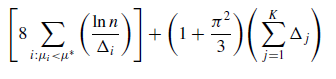
\includegraphics[scale=0.7]{img/theorem.png}
\end{tabbing}
where $\mu_{1}, . . . , \mu_{K}$ are the expected values of $P_{1}, . . . , P_{K}$ .
\end{theorem}
\end{frame}

%------------------------------------------------

%------------------------------------------------
\begin{frame}
\frametitle{UCB 1 Proof}

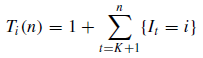
\includegraphics[scale=0.7]{img/line1.png}
Initially each arm has been pulled once. So from K+1 th attempt till n we are trying to bound $T_{i} (n)$

\begin{tabbing}
\hspace*{.25in}
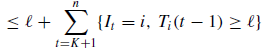
\includegraphics[scale=0.7]{img/line2.png}
\end{tabbing}

We have played arm i at least $\ell$ number of times till t-1 th time indicated by $T_{i}(t-1)$. This means that the arm i pulled till time n will be less than equal to some arbitrary positive integer $\ell$

\begin{tabbing}
\hspace*{.25in}
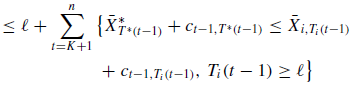
\includegraphics[scale=0.7]{img/line3.png}
\end{tabbing}

Since we are pulling this arm i again this means that the UC of optimal arm(l.h.s) is less than the UC of the i th arm(r.h.s) given that the number of times the arm i is pulled till time t-1 is atleast greater than $\ell$. 

\end{frame}

\begin{frame}
\frametitle{UCB 1 Proof}
The Upper confidence bound is given by the mean of the reward and the confidence interval term of that arm. This confidence interval term $c_{t}$ we will derive later by the Chernoff-Hoeffding bound.

\begin{tabbing}
\hspace*{.25in}
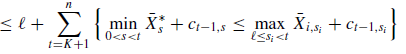
\includegraphics[scale=0.7]{img/line4.png}
\end{tabbing}

For atleast once the minimum of the UC of the optimal arm from 0 - t th time is less than the maximum of the UC of the i th arm from $\ell$ to t th time. Here the number of times the optimal arm is pulled is denoted by s and for the ith arm denoted by $s_{i}$

\begin{tabbing}
\hspace*{.25in}
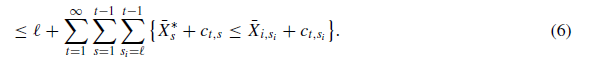
\includegraphics[scale=0.7]{img/line5.png}
\end{tabbing}

Summing over all pulls from the start. 
\end{frame}

\begin{frame}
\frametitle{UCB 1 Proof}
\begin{tabbing}
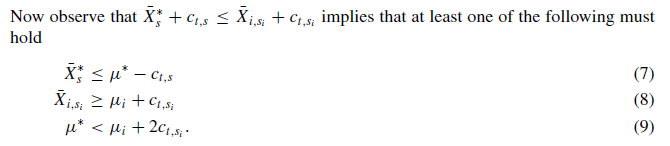
\includegraphics[scale=0.7]{img/observe.png}
\end{tabbing}

\end{frame}

%------------------------------------------------

%------------------------------------------------
\begin{frame}
\frametitle{UCB 1 Proof}
These three conditions are shown below

\begin{tabbing}
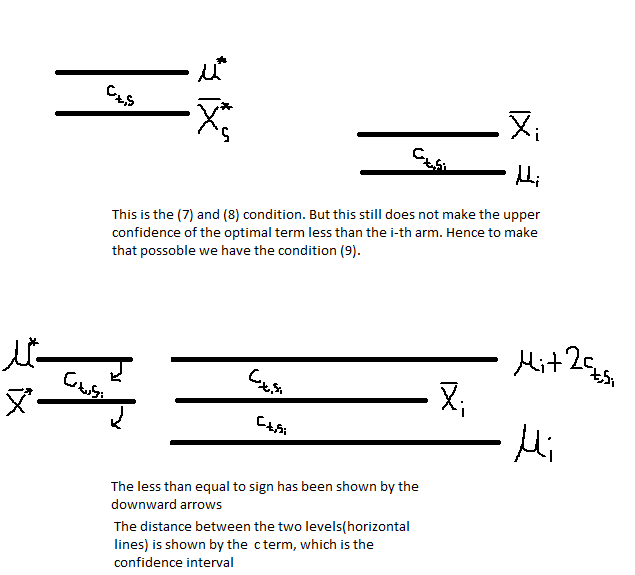
\includegraphics[scale=0.3]{img/Explanation.png}
\end{tabbing}
\end{frame}

%------------------------------------------------

\begin{frame}
\frametitle{UCB 1 Proof}

From the (9) condition we can definitely show that $\overline{X}_{s}^{*}$ is less than $\overline{X}_{i}$.
\newline
\newline
Next, we bound the probability of events (7) and (8) using Fact 1(Chernoff-Hoeffding bound)
\newline
For (7)
$\mathbb P\lbrace\overline{X}_{s}^{*}\leq\mu^{*}-c_{t,s}\rbrace \leq e^{-2c_{t,s}^{2}/s} \leq e^{-4lnt} = t^{-4}$ by putting $c_{t,s}=\sqrt{2lnt/s}$
\newline
For (8)
$\mathbb P\lbrace\overline{X}_{i,s_{i}}\geq\mu_{i}+c_{t,s_{i}}\rbrace \leq e^{-2c_{t,s_{i}}^{2}/s_{i}} \leq e^{-4lnt} = t^{-4}$ by putting $c_{t,s_{i}}=\sqrt{2lnt/s_{i}}$
\newline

Now, for $\ell=\lceil (8ln n)/\Delta_{i}^{2}\rceil$ (9) is false. This can be proved by putting this $\ell$ value in
\newline
$\mu^{*} - \mu_{i} - 2c_{t,s_{i}}= \mu^{*} - \mu_{i} - 2\sqrt{2ln t/s_{i}}=\mu^{*} - \mu_{i} - 2\sqrt{2ln t\Delta_{i}^{2}/(8lnt)}=\mu^{*} - \mu_{i} - \Delta_{i} = \mu_{*} - \mu_{i} - \mu_{*} + \mu_{i}=0$
\newline
by putting $\Delta_{i}=\mu_{*} - \mu_{i}$ above.

Next, in (6) we put the value of $\ell$ and the conditions which satisfies the necessary upper confidence bounds.

\end{frame}

%------------------------------------------------

\begin{frame}
\frametitle{UCB 1 Proof}
\begin{tabbing}
\hspace*{.25in}
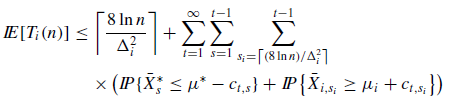
\includegraphics[scale=0.7]{img/line6.png}
\end{tabbing}

\begin{tabbing}
\hspace*{.25in}
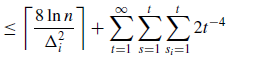
\includegraphics[scale=0.7]{img/line7.png}
\end{tabbing}

The inequality comes because we are summing over all all instances from s=1 to t-1 rather than only from $\ell$
\newline
$\leq \lceil \frac{8ln n}{\Delta_{i}^{2}}\rceil + \Sigma_{t=1}^{\infty}2t^{-4}\Sigma_{s=1}^{t}\Sigma_{s_{i}=1}^{t}(1)$ 
\newline
$\leq  \frac{8ln n}{\Delta_{i}^{2}} + 1 + \Sigma_{t=1}^{\infty}2t^{-4}t^{-2}$ [Removing the ceiling]
\newline
$\leq  \frac{8ln n}{\Delta_{i}^{2}} + 1 + \Sigma_{t=1}^{\infty}2t^{-2}$
\newline
$\leq  \frac{8ln n}{\Delta_{i}^{2}} + 1 + 2\times\frac{\pi^{2}}{6}$ from Basel's Equation

\end{frame}

%------------------------------------------------

\begin{frame}
\frametitle{UCB 1 Proof}
\begin{tabbing}
\hspace*{.25in}
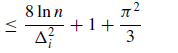
\includegraphics[scale=0.7]{img/line8.png}
\end{tabbing}

This concludes the proof.
\end{frame}

%------------------------------------------------

\begin{frame}
\frametitle{UCB 1 Experimental Run}
%\begin{tabbing}
\begin{center}
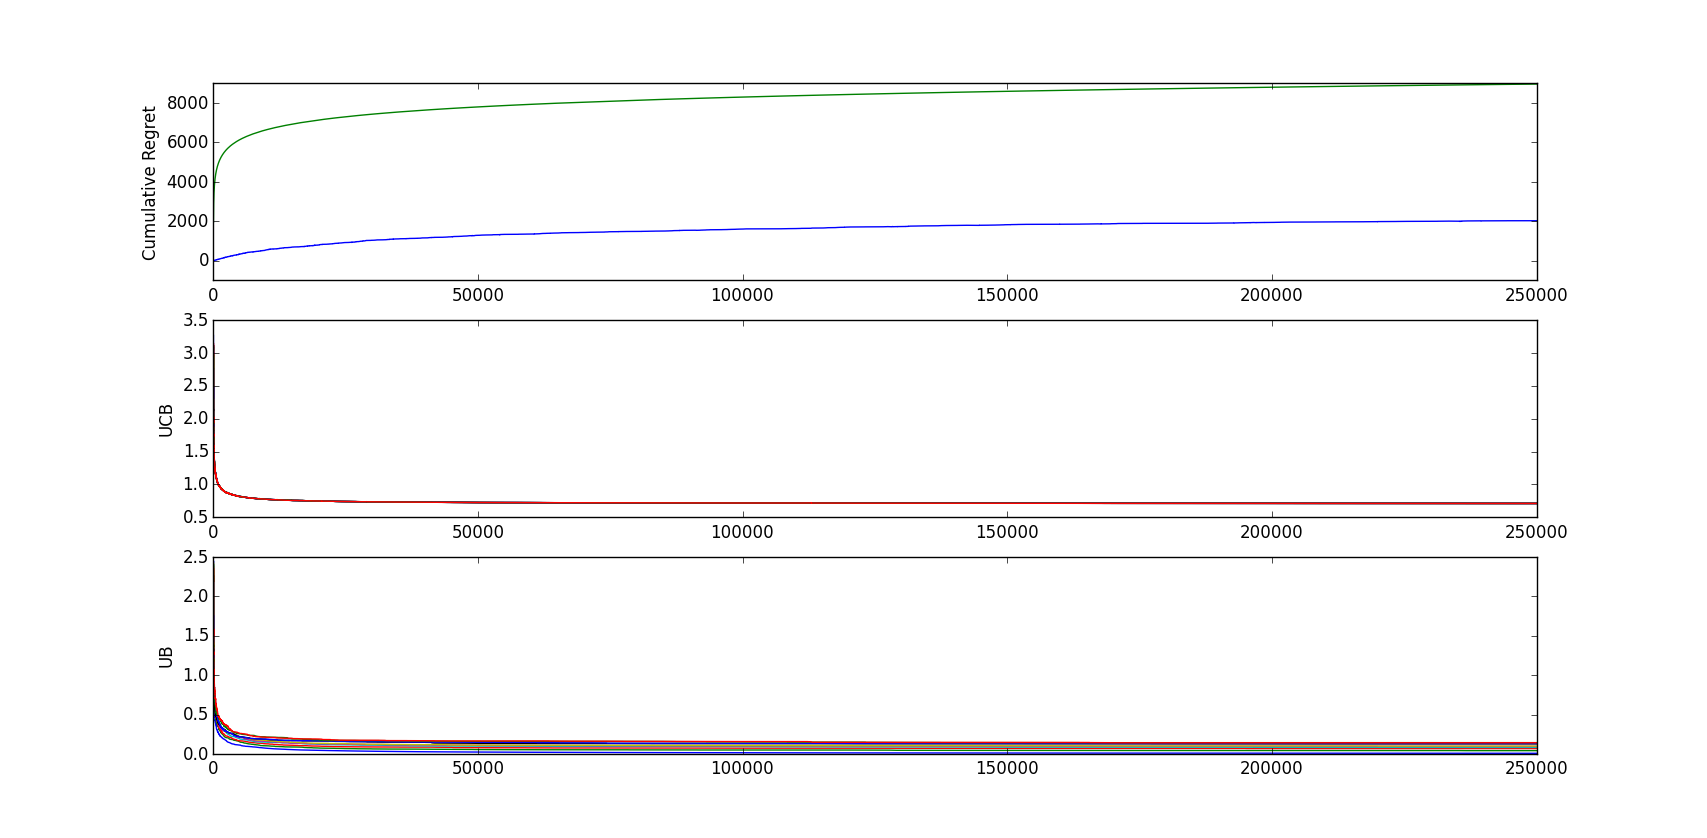
\includegraphics[scale=0.3]{img/ucb.png}
\end{center}

%\end{tabbing}
\end{frame}

%------------------------------------------------

\begin{frame}
\frametitle{Some Other Bandits and Applications}

\begin{itemize}
\item Adversarial Bandits : Used in Investment in Stock Markets
\item Contextual Bandits : Used in online Advertisement/news article selection
\item Budgeted Bandits : Used in Clinical trials
\item Distributed Bandits : Used in packet routing through a network
\end{itemize}

\end{frame}

%------------------------------------------------

%\begin{frame}
%\frametitle{References}
%\footnotesize{
%\begin{thebibliography}{99} % Beamer does not support BibTeX so references must be inserted manually as below
%\bibitem[PETER AUER,NICOL`O CESA-BIANCHI,PAUL FISCHER 2002]{p1} PETER AUER,NICOL`O CESA-BIANCHI,PAUL FISCHER (2002)
%\newblock Finite-time Analysis of the Multiarmed Bandit
%Problem
%\newblock \emph{Machine learning} 47,2-3, 235--256.
%
%%\begin{thebibliography}{99} % Beamer does not support BibTeX so references must be inserted manually as below
%\bibitem[Auer, Peter and Ortner, Ronald 2010]{p1} Auer, Peter and Ortner, Ronald (2010)
%\newblock UCB revisited: Improved regret bounds for the stochastic multi-armed bandit problem
%Problem
%\newblock \emph{Periodica Mathematica Hungarica} 61,1-2, 55--65.
%
%\bibitem[Sutton and Barto 1988]{p1} Sutton and Barto (1988)
%\newblock Reinforcement Learning: An Introduction
%%\newblock \emph{Periodica Mathematica Hungarica} 61,1-2, 55--65.
%\end{thebibliography}
%}
%\end{frame}

\begin{frame}
\frametitle{References}
\bibliographystyle{plainnat}
\bibliography{biblio}
\end{frame}




%------------------------------------------------

\begin{frame}
\Huge{\centerline{Thank You}}
\end{frame}

%----------------------------------------------------------------------------------------

\end{document} 